\chapter{Introduction} \label{cha:intro}

The years 2004 through 2006 mark an interesting shift in the world of computing: Single threaded performance growth has slowed down significantly since that period in time when CPU architectures arrived at their thermal design limits. Where single threaded floating point performance would grow by 64\% per year before, it only gains roughly 21\% per year since then~\cite{SingleThreadCPUPerf}. This lead to a paradigm shift towards more parallelism on the socket level, a development for which Graphics Processors, out of necessity, have always been at the forefront. 

In recent years there has been a push in the high performance computing (HPC) community into using Graphics Processing Units for General Purpose (GPGPU) Computing. The Tokyo Institute of Technology's TSUBAME 2.0 Supercomputer (currently ranking 14th in the TOP500 list~\cite{TsubameTop500}) is a prime example of this development. 

The GPU instruction sets - and in extent the software development models - have not yet come to a point where they are generally applicable to programs orignally written for CPUs without significant restructurings however. Key players of the HPC industry have at the end of 2011 pushed towards a higher level programming model for GPUs through the \textquotedblleft OpenACC\textquotedblright\ standard, and their compilers have now reached a point where this new GPGPU programming model becomes of interest for HPC software development.

\section{Structure of this Thesis}

In this thesis the applicability of GPGPU computing to the physical core of Japan's next generation weather prediction model \textquotedblleft ASUCA\textquotedblright\ will be examined in light of these recent developments in GPGPU programming models (cha.~\ref{cha:evaluation}). A suitable high performance toolset based on these examinations will be developed for this usecase with possible applications in other areas of scientific computing (cha.~\ref{cha:framework}, cha.~\ref{cha:implementation}). The usability and performance of this framework will be verified (cha.~\ref{cha:analysis}), before pointing out the achievements and future work of this thesis (cha.~\ref{cha:achievements}).

The following chapter will describe the ASUCA weather prediction model (sec.~\ref{sec:modelASUCA}), state the motivation and goals for this thesis (sec.~\ref{sub:thesisMotivation}), introduce the key technologies and terms used throughout (sec.~\ref{sec:fermi}) and point to related work (sec.~\ref{sec:relatedWork}).

% for desktop computers which soon began influencing the world of high performance computing as well, where massively parallel execution has always been key. Commodity hardware has already replaced custom vector processors in the \textquotedblleft Attack of the Killer Micros\textquotedblright\ ~\cite{attackOfKillerMicros} during the 1990ies. Now the 

\section{ASUCA Weather Prediction Model} \label{sec:modelASUCA}

The Japan Meteorological Agency (JMA) currently operates a nonhydrostatic~\footnote{Nonhydrostatic as in the opposite of models using the hydrostatic approximation, i.e. the entire vertical momentum equation is being kept in the model~\cite[p. 138]{jacobsonAtmosphereFundamentals}.} regional weather prediction model called \textquotedblleft JMANHM\textquotedblright. This model has been used since the 1990s. The rapid increase of parallel architectures on the socket level, as mentioned in the preface, have lead to the motivation to renovate the weather model in order to make best use of these new levels of parallelism~\cite[p. 3]{KawanoASUCA}.

The new nonhydrostatic model, to be called \textquotedblleft ASUCA\textquotedblright\footnote{\textbf{A}SUCA is a \textbf{S}ystem based on a \textbf{U}nified \textbf{C}oncept for \textbf{A}tmosphere.}, is being developed with the following objectives~\cite[p. 1]{ASUCA2010},\cite[p. 4]{KawanoASUCA}: 
\begin{enumerate}
 \item Higher accuracy.
 \item Higher efficiency.
  \begin{enumerate}
   \item Less data communication.
   \item Suitable to the current computer architecture.
  \end{enumerate}
\end{enumerate}

ASUCA uses a three-dimensional, horizontally and vertically staggered grid~\footnote{The type of grid used for ASUCA is called ``Arakawa C'', also being used by the European Consortium for Small Scale Modeling (COSMO) for the weather prediciton model of multiple European nations~\cite[p. 4]{baldaufWetterdienstCourse}.}, consisting of the two relatively widely spaced horicontal dimensions $I$ and $J$ and the densely spaced vertical dimension $K$. The equations are discretized using the finite volume method (FVM).~\cite[p. 2]{Shimokawabe2010}

\begin{figure}[htpb]
	\centering
	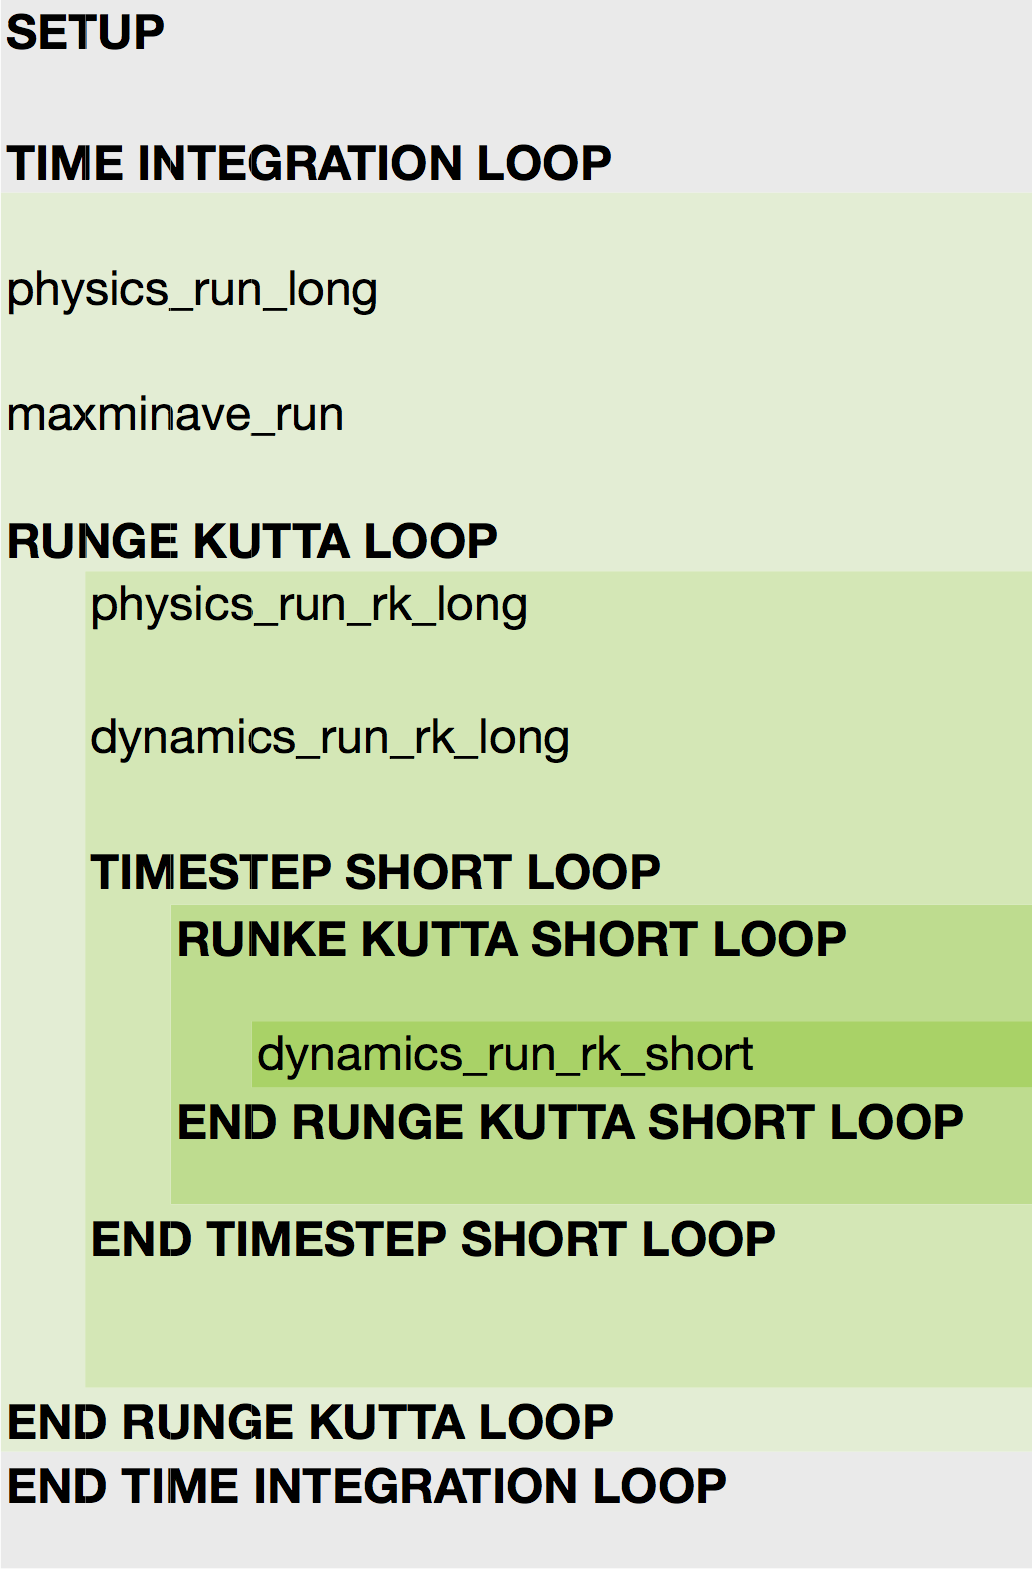
\includegraphics[width=6cm]{figures/arashiOverview}
	\caption[Overview ASUCA Model Program Flow]{Overview ASUCA Model Program Flow.}
	\label{figure:arashi}
\end{figure}

Fig.~\ref{figure:arashi} gives an overview over the program flow in the ASUCA model. Physical and dynamical processes\footnote{``Physical'' processes can be understood as in they produce input parameters for the dynamical processes based on the last timestep's dynamics results, boundary conditions and constant factors.} are executed for each timestep. Each long timestep also contains a short time integration loop for processes that require a higher time resolution\footnote{Horizontal sound wave and gravity wave propagation.}. These short timestep processes also employ a second-order Runge-Kutta scheme as depicted in the figure.~\cite[p. 2]{Shimokawabe2010}

\section{Motivation and Goal of Thesis} \label{sub:thesisMotivation}

The dynamical core (containing the dynamical processes depicted in fig.~\ref{figure:arashi}) was already extended for the GPU using CUDA C~\footnote{See sec.~\ref{sub:cudaIntro}.} by Shimokawabe et al.~\cite[p. 2]{Shimokawabe2011} 

Consequently, the next task will be the development of algorithms for the physical processes suitable for GPGPU computing. The main \textbf{motivation} for this development is to 
\begin{enumerate}
 \item eliminate host-to-device communication during the entire time integration loop.
 \item gain speedups in execution time. 
\end{enumerate}
Being able to run this process faster on the same amount of computing nodes by employing GPGPU technology would lead to cost and energy savings and possibly an increased grid resolution, giving the model a higher accuracy.

 The following \textbf{characteristics} can be observed about the dynamical in comparison to the physical core: 
\begin{enumerate}
 \item The dynamical core accounts for a higher fraction of the runtime.
 \item The dynamical core employs less lines of code.
 \item The dynamical core tends to be more ``stable'' over time, i.e. the dynamical processes are not under constant development while this is the case for various physical modules. 
\end{enumerate}

For these reasons the dynamical processes are a prime candidate for deep performance optimizations, while porting the physical processes brings different \textbf{challenges}: 

\begin{itemize}
 \item How can the physical processes be ported while keeping a familiar development environment for the JMA researchers, i.e. Fortran 90? 
 \item How can the physical processes be ported with the least amount of code changes compared to the current code? 
 \item How can the physical processes be ported to the GPU while still keeping the code executable on CPU?
 \item How can all of the above be achieved while still enabling a high GPU performance?
 \item How can the CPU performance of the hybridized code be kept at the same level as with code that has been specifically optimized for the CPU? This would enable a heterogenous execution of the code on systems with both highly capable CPU and GPU resources such as TSUBAME 2.0. Specifically for the case of JMA's ASUCA this is a very important aspect, since it is planned to gradually move towards GPU execution while still maintaining CPU compatibility.  
\end{itemize}

The \textbf{main goal for this thesis} is to find and verify a strategy with which the questions above can be answered. In this thesis single socket parallelism will be discussed. Multi socket / multi node parallelism will be solved through MPI communication, which will not be covered here.

% \section{Domain Knowledge Assumed in this Thesis}
% CUDA syntax
% Fortran 90 syntax
% OpenACC syntax

\clearpage
\section{GPGPU Computing on the NVIDIA Fermi Architecture} \label{sec:fermi}

The Tokyo Institute of Technology's TSUBAME 2.0 Supercomputer has been used as a development and test platform. This system currently uses NVIDIA Fermi\footnote{The Fermi architecture has been introduced in 2010 and has been highly popular in the HPC world, in part because of high double precision performance and support for ECC Memory. Four systems in the current top 20 use Fermi cards~\cite{Top500}.} based GPUs, of which three are added to each computing node, as well as \textquotedblleft Westmere\textquotedblright\ generation Intel Xeon CPUs. More details about the hardware specifications and models can be found in sec.~\ref{sec:testHardware}.

When it comes to GPGPU software library and tooling support, NVIDIA's Fermi GPU architecture is currently regarded as the most mature. Therefore, this thesis mainly concentrates on the available software technologies for NVIDIA GPUs on TSUBAME 2.0. However, it must be noted that vendor independant solutions would naturally be of an advantage - something that will be kept in mind for later conclusions.

\subsection{NVIDIA Fermi} \label{sub:fermi}

\begin{figure}[hbtp]
  \centering  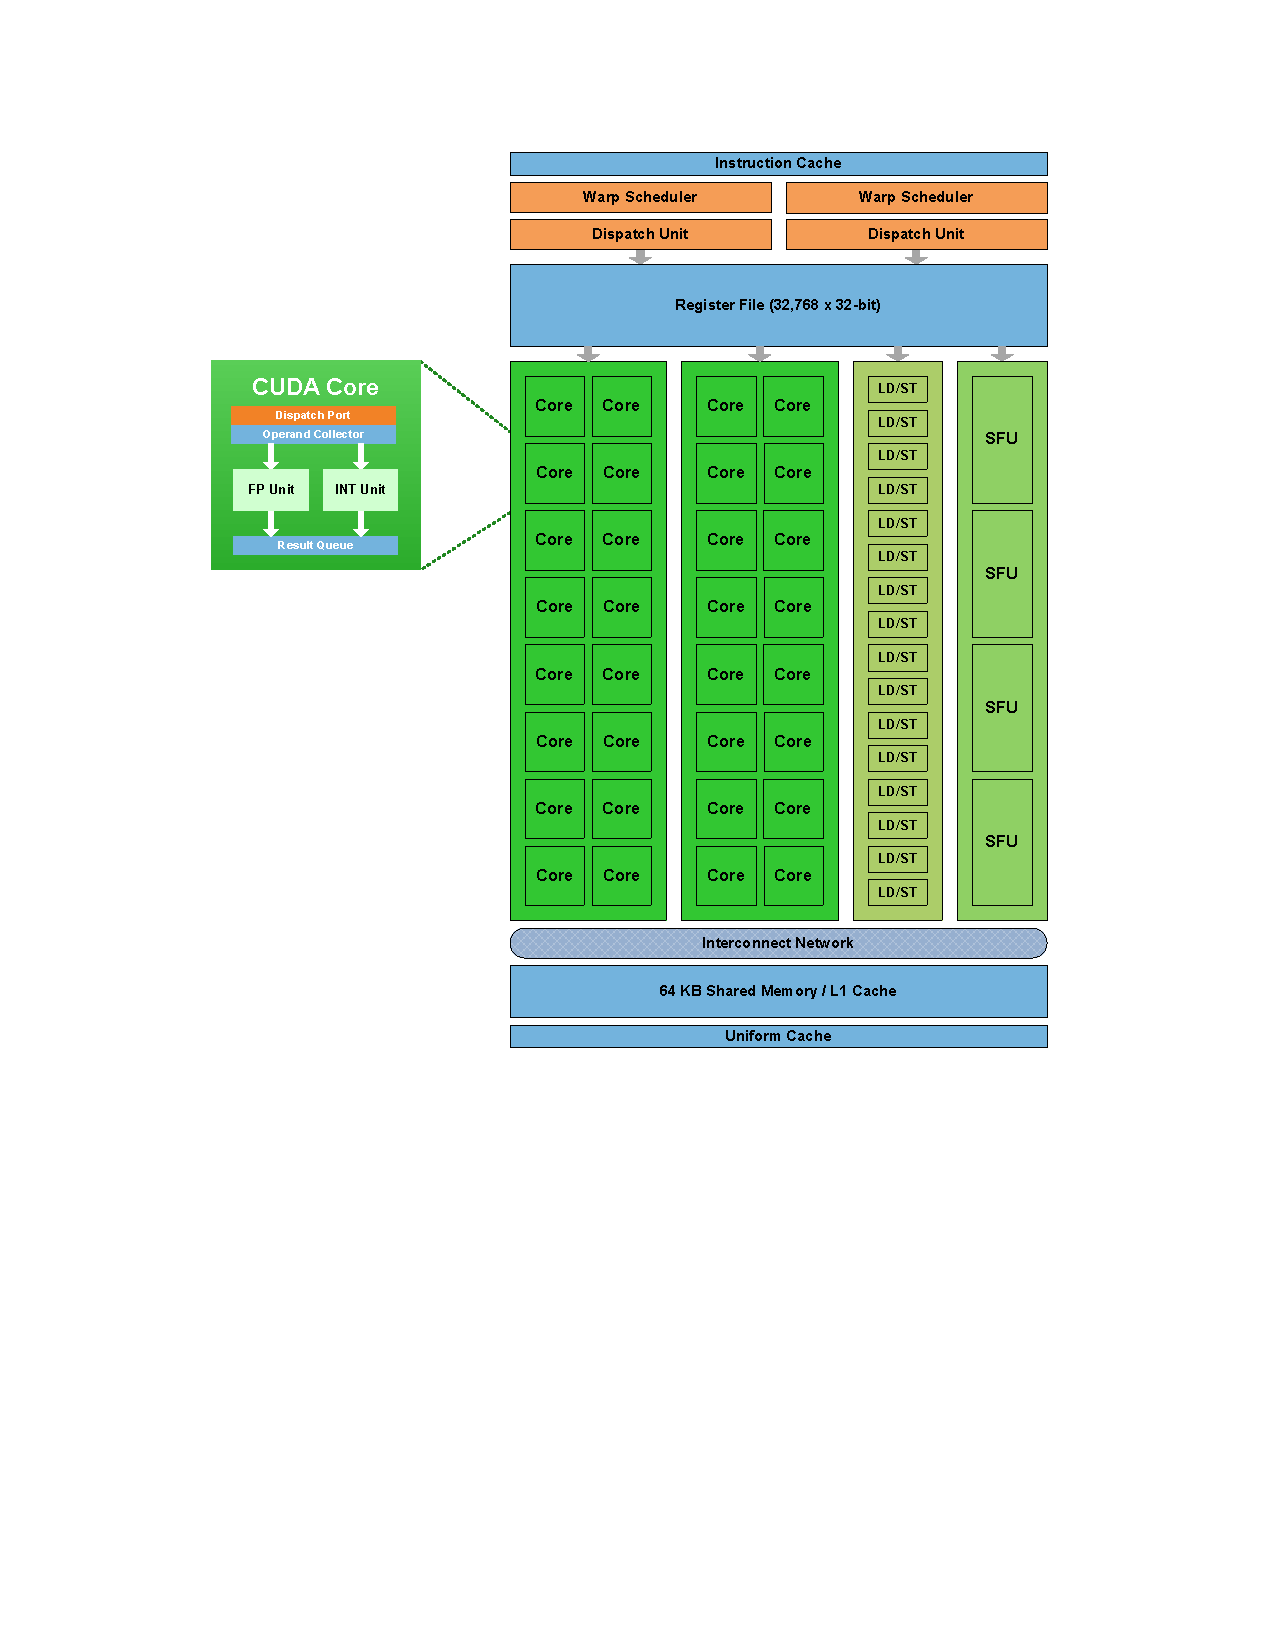
\includegraphics[width=10cm]{figures/FermiOneSM.pdf}
  \caption [Layout of One Streaming Multiprocessor (SM)]{One SM contains 32 computational cores, 16 load/store units, 4 \textquotedblleft Special Function\textquotedblright\ units, 32'768 4-byte-registers and 64kB L1 cache / Shared memory~\cite[p. 8]{FermiWhitepaperOfficial}.}
  \label{figure:fermiOneSM}
\end{figure} 

The main difference between CPU and GPU computing lies in the GPU's massively parallel nature. NVIDIA Fermi employs 16 so called \textquotedblleft Streaming Multiprocessors\textquotedblright\ (SMs) with 32 computing cores each, resulting in 512 threads running in parallel\footnote{The number of possible threads is half of that number for double precision execution in case of Tesla branded Fermi GPUs, significantly lower even for the GeForce brands.}. Each core, naturally, has a much lower complexity than any x86 core, which is reflected in the reduced scheduler, cache and register resources available to it. Figure \ref{figure:fermiOneSM} shows the ressources of one SM.  

The following hardware characteristics are very important when it comes to discussing the programming model: 
\begin{enumerate}
 \item GPUs employ a scheduling scheme similar to SIMD\footnote{\textbf{S}ingle \textbf{I}nstruction \textbf{M}ultiple \textbf{D}ata, the classic scheme for vector processors.}: Each instruction is executed by a number of threads multiple of 32 (up to 512 in Fermi's case) for a whole block of data. However, compared to SIMD, these threads can be scheduled more freely, e.g. allowing branching\footnote{Branches will however degrade the performance of GPU code, since only one code path of the branch will be executed in parallel - threads that are not in that path will simply execute \textquotedblleft nop\textquotedblright\ instructions during that time.}. The memory architecture is optimized for coalesced loads / stores of data blocks with a multiple of $32\times4$ byte size. A 32 thread unit, reflected in the SM architecture, is thus very important for Fermi GPGPU computing, and is being called \textquotedblleft Warp\textquotedblright.
 \item The cost of thread context switching is orders of magnitude lower than on x86, to a point where it becomes negligible for most use cases. 
\end{enumerate}

\subsection{CUDA Programming Model} \label{sub:cudaIntro}

\textquotedblleft Compute Unified Device Architecture\textquotedblright\ (CUDA) is an integrated hardware and software technology developed by NVIDIA for writing general purpose programs on their GPUs. Since thread switching is very cheap, as discussed in sec.~\ref{sub:fermi}, CUDA programs are usually written in a way, such that for every data point in the parallel domain one thread (or a series of threads, executed sequentially) is created. Threads are bundled into one-, two- or three dimensional thread blocks, such that each block is executed on one SM. One of the first tasks when adapting a program for CUDA, is usually to map the involved data structures onto threadblocks, such that memory reads can be optimized into coalesced fetches of at least $32\times4$ bytes. This is usually accomplished using simple one dimensional or multi dimensional arrays.

CUDA Programs consist of the following parts: 

\begin{description}
 \item [Host code] is code that will be executed on the host system CPU(s). It is being compiled through third party compilers, with NVIDIA providing a runtime library for interactions with the device\footnote{In GPGPU Computing, the word \textquotedblleft device\textquotedblright\ is generally used for the GPU.}, such as device memory allocations, device data transfer and kernel calls. 
 \item [Kernel functions] define the program of one GPU thread. Memory access is usually specified by using an index that encodes thread ID and block ID of one thread. In conventional programming terms, CUDA kernel definitions best correspond to parallelizable \verb|for| loops.
 \item [Device functions] define subroutines that can be called from a Kernel function. These subroutines need to be inlineable by the CUDA compiler.
\end{description}

Kernels (including the inlined device functions) will be compiled to an intermediate device code representation called \textquotedblleft PTX\textquotedblright\ through the CUDA compiler.

\subsection{OpenACC Programming Model} \label{sub:openACCIntro}

OpenACC is a relatively new standard introduced in 2011, with the intention to bring the power of directive based parallelization, such as OpenMP, to GPGPU computing~\cite{beyerOpenMPforAcc}. The standard has been developed by CAPS, Cray and The Portland Group in association with NVIDIA~\cite{nvidiaOpenACC}. Before the OpenACC standardization, the aforementioned companies each developed their own proprietary GPU parallelization directives for their compiler solutions. Current OpenACC compilers only support NVIDIA CUDA implementations of OpenACC user code.

The main functionality of OpenACC is the abstraction of GPU kernels through directives added to \verb|for| loops (\verb|do| loops in case of Fortran code). Adding such directives delegates the responsibility of implementing a GPU kernel to the {OpenACC} compiler. As an added benefit, the codebase becomes hybrid, i.e. executable on both CPU and GPU. Device data handling is solved through additional directives.

\clearpage
\section{Related Work} \label{sec:relatedWork}

\begin{description}
 \item [Naoya Maruyama, Tatsuo Nomura et al.] \textit{Physis: An Implicitely Parallel Programming Model for Stencil Computations on Large-Scale GPU-Accelerated Supercomputers}: This paper describes a compiler-based programming framework that automatically translates user-written structured grid code into a parallel implementation code for multi-GPUs, using a DSL embedded in C language code.~\cite{Maruyama}
 
 \item [Tobias Gysi (Super Computing Systems AG)] \textit{A Stencil Library for the New Dynamic Core of COSMO}: This talk examines the stencil DSL library that has been developed for the European Consortium for Small Scale Modeling (COSMO), the maintaining gremium of the climate model for seven European countries. This stencil DSL library heavily relying on C++ templates has been applied to the Dynamical Core of the COSMO model and enables hybrid execution on CPU and GPU.~\cite{Gysi}
 
 \item [Takashi Shimokawabe, Takayuki Aoki et al.] \textit{An 80-Fold Speedup, 15.0 TFlops Full GPU Acceleration of Non-Hydrostatic Weather Model ASUCA Production Code}: This paper examines the portation of the dynamical core of the ASUCA weather prediction model to GPGPUs on TSUBAME 1.2 (Tesla S1070, AMD Opteron). Single GPU vs. single core CPU execution achieved a speedup of 26.3 in double precision. The multi-GPU implementation achieved an overall single precision performance of 15.0 TFlops on only 528 GPUs - a remarkable achievement compared to the 50 TFlops record at that time on more than 18'000 Jaguar nodes with nearly 150'000 CPU cores. To achieve this performance, optimization methods for overlapping communication and computation, as well as asynchronous computation of variables were explored.~\cite{Shimokawabe2010}
 
 \item [Takashi Shimokawabe, Takayuki Aoki et al.] \textit{145 TFlops Performance on 3990 GPUs of TSUBAME 2.0 Supercomputer for an Operational Weather Prediction}: This paper examines the results of the ASUCA dynamical core portation, first introduced in \cite{Shimokawabe2010}, applied to the TSUBAME 2.0 architecture. Single precision performance improved by 10\% while double precision performance improved by 65\% on single Tesla M2050 compared to the Tesla S1070 of TSUBAME 1.0. On multi-GPUs, 145 single precision TFlops on 3990 GPUs and 76.1 double precision TFlops on 3936 GPUs have been achieved. As a future real world application, a typhoon over Japan has been simulated on a very high mesh resolution of 500m.~\cite{Shimokawabe2011}
 
 \item [John Michalakes, Manish Vachharajani] \textit{GPU Acceleration of Numerical Weather Prediction}: In this paper Michalakes and Vachharajani describe the GPU portation of the so-called WRF\footnote{``The Weather Research and Forecast'' model, the world's most widely used weather prediction model.} Single Moment 5-tracer (WSM5) module using NVIDIA CUDA C. This lead to a $7.7\times$ performance increase for that module and $1.23\times$ performance increase for the overall WRF model.~\cite{Michalakes}
 
 \item [John C. Linford, John Michalakes et al.] \textit{Multi-core Acceleration of Chemical Kinetics for Simulation and Prediction}: In this paper the implementation of a computationally expensive chemical kinetics kernel was compared on three multicore platforms: NVIDIA Tesla C1060 GPUs, Cell Broadband Engine (CBEA) and Intel Quad-Core Xeon. The CBEA achieved the highest speedup of $41.1\times$ compared to the serial implementation in single precision. The GPU architecture was hampered because of low availability of on-chip memory and achieved a speedup of only $8.5\times$ compared to the serial implementation in single precision.~\cite{Linford}
 
 \item [Stefan Kronig, Michel M\"{u}ller] \textit{Feasibility and Performance of Weather Computations using GPGPU Programming}: This semester thesis, conducted in collaboration with Tobias Gysi of Super Computing Systems AG, contains a preliminary examination for a GPU port of the Dynamical Core of the COSMO Weather model, using a sample algorithm.~\cite{MuellerKronig}
\end{description}
